\input ../SlidePreamble
\input ../preamble


\begin{document}

{\Huge

  \centerline{\bf TTIC 31230, Fundamentals of Deep Learning}
  \bigskip
  \centerline{David McAllester, Autumn 2022}
  \vfill
  \vfil
  \centerline{Diffusion Model Basics}
  \vfill
  \vfill

\slidetwo{Denoising Diffusion Probabilistic Models}{Ho, Jain and Abbeel, June 2020}

\centerline{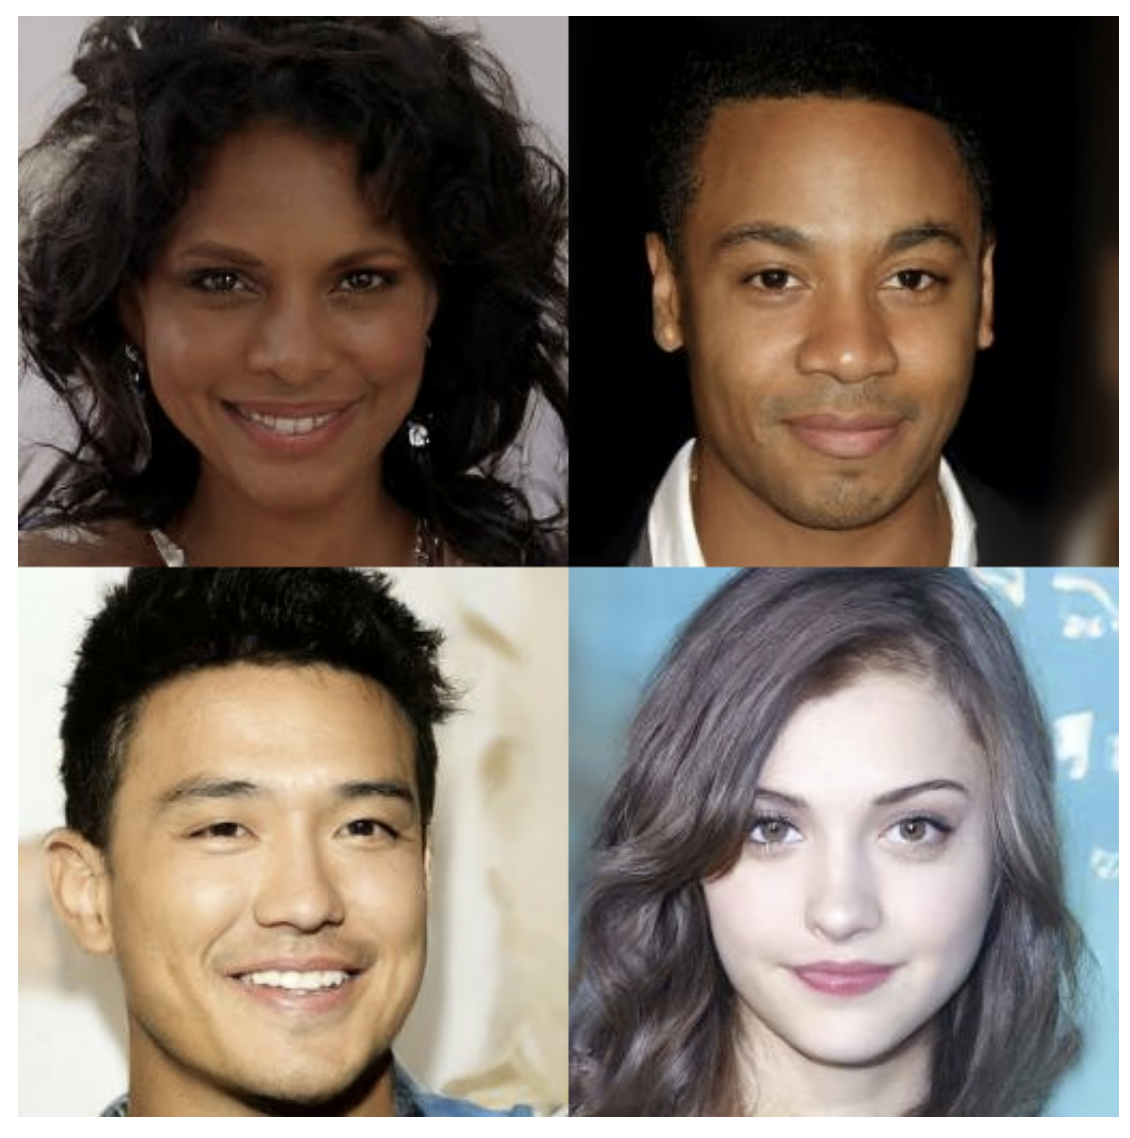
\includegraphics[width = 4in]{\images/DiffCeleb}}


\slide{Progressive VAEs}

Diffusion models are a special case of progressive VAEs.

\vfill
A progressive VAE has layers of latent variables $z_1,\dots,z_{L}$.

\vfill
The encoder defines $P_{\enc_0}(z_1|y)$ and $P_{\enc_\ell}(z_{\ell+1}|z_\ell)$ (defining a Markov chain).

\vfill
We have a prior $P_\pri(z_L)$ and a decoder defined by $P_{\dec_\ell}(z_{\ell}|z_{\ell+1})$ and $P_{\dec_0}(y|z_1)$.

\vfill
Ho et al. take {\color{red} $L = 1000$.}

\slide{The Ho et al. Diffusion Model}

The encoder is not trained --- The encoder just adds noise.

\vfill
The encoder is designed so that $Z_L$ is distributed as ${\cal N}(0,I)$.  The prior is not trained.

\vfill
The decoder is a single network applied to all layers but taking the layer as an argument.

\slide{A Gaussian Noise Encoder}

We assume $y \in R^d$ and $z_\ell \in R^d$.

\vfill
In the case of images every $z_\ell$ is an image with the same dimension as $y$.

\vfill
For notational convenience we define $z_0 = y$.

\vfill
The index $\ell$ will always range from $1$ to $L$ where $z_{\ell-1}$ might be $z_0$.

\vfill
The encoder is fixed (not trained) and is defined by a sequence of noise levels $\sigma_1$, $\ldots$, $\sigma_L$ where for $1 \leq \ell \leq L$ we have

$$z_\ell = \sqrt{1-\sigma^2_\ell}\;z_{\ell-1} + \sigma_\ell \epsilon\;\;\;\;\epsilon \sim {\cal N}(0,I)$$

\slide{A Gaussian Noise Encoder}

$$z_\ell = \sqrt{1-\sigma^2_\ell}\;z_{\ell-1} + \sigma_\ell \epsilon\;\;\;\;\epsilon \sim {\cal N}(0,I)$$

\vfill
This is designed so that if $z_\ell$ as unit variance in each dimension then $z_{\ell+1}$ also has unit variance in each dimension.

\vfill
$z_0 = y$ is scaled so that each coordinate is in the interval $[0,1]$.

\vfill
The constant variance of $z_\ell$ is important because the same decoder is being used at all $\ell$ and we want
the scale of the decoder input to be independent of $\ell$.

\slide{A Gaussian Noise Encoder}

$$z_\ell = \sqrt{1-\sigma^2_\ell}\;z_{\ell-1} + \sigma_\ell \epsilon\;\;\;\;\epsilon \sim {\cal N}(0,I)$$

\vfill
Note that the mean of $z_\ell$ equals $\sqrt{1-\sigma_\ell}$ times the mean of $z_{\ell-1}$.

\vfill
This repeated reduction drives the mean of $z_L$ to a negligible level.

\vfill
We then get that $z_L$ is distributed as ${\cal N}(0,I)$.

\slide{A Gaussian Noise Encoder}

$$z_\ell = \sqrt{1-\sigma^2_\ell}\;z_{\ell-1} + \sigma_\ell \epsilon\;\;\;\;\epsilon \sim {\cal N}(0,I)$$

\vfill
They increase the noise at higher levels.  After some experimentation they use

$$\sigma^2_\ell = 10^{-4} + .02\;\frac{\ell}{L}\;\;\;(\mbox{with $L = 1000$)}$$



\slide{Direct Sampling of $z_\ell$}

We can sample from $P_\enc(z_\ell|z_0)$ directly

$$\mbox{define}\;\;\;\alpha_\ell = \prod_{\ell = 1}^\ell \sqrt{1-\sigma^2_\ell}$$

\vfill

$$z_\ell = \alpha_\ell z_0 + \sqrt{1-\alpha^2_\ell} \;\epsilon\;\;\;\epsilon \sim {\cal N}(0,I)$$

\vfill
The variance of the noise term can be derived by solving a recurrence relation or by observing that $z_\ell$ must have unit variance for unit variance $z_0$.

\slide{A Natural but Problematic Loss Function}

$$\dec^* = \argmin_{\dec}\;\;E_{z_0,\ell,z_{\ell-1},z_\ell} \;\;||z_{\ell-1} - \dec(z_\ell,\ell)||^2$$

\vfill
Here $z_{\ell-1}$ is sampled directly from $z_0$ and $z_\ell$ is sampled from $z_{\ell-1}$.

\slide{Reducing the Decoder's Dependence on $\ell$.}

We have already reduced the decoder's dependence on $\ell$ by making $z_\ell$ have unit variance for all $\ell$.

\vfill
But predicting $z_{\ell-1}$ from $z_\ell$ behaves differently for different $\ell$.

\vfill
For small $\ell$, where $\sigma_\ell$ is small, $z_{\ell-1}$ is near $z_\ell$.
For large $\ell$ we have that $z_{\ell-1}$ is far from $z_\ell$.  Since the same network is used at all $\ell$ we want to reduce the dependence on $\ell$.

\vfill
This can be accomplished by using an $\epsilon$-decoder.

\slide{An $\epsilon$-Decoder}

First we solve for $z_{\ell-1}$ in terms of $z_\ell$ and $\epsilon$.

$$z_\ell = \sqrt{1-\sigma^2_\ell}\;z_{\ell-1} + \sigma_\ell \epsilon\;\;\;\;\epsilon \sim {\cal N}(0,I)$$

\vfill
$$z_{\ell-1} = \frac{1}{\sqrt{1-\sigma_\ell^2}}(z_\ell - \sigma_\ell \epsilon)$$

\vfill
$$\dec(z_\ell,\ell) = \frac{1}{\sqrt{1-\sigma_\ell^2}}\left(z_\ell - \sigma_\ell\; \epsilon_\Phi(z_\ell,\ell)\right)\; +\; \sigma_\ell\delta\;\;\;\;\;\delta \sim {\cal N}(0,I)$$

\vfill
Here $\epsilon_\Phi(z_\ell,\ell)$ is a trained network whose target value has the same behavior at all levels of $\ell$.

\slide{An $\epsilon$-Decoder}

$$\dec(z_\ell,\ell) = \frac{1}{\sqrt{1-\sigma_\ell^2}}\left(z_\ell - \sigma_\ell\; \epsilon_\Phi(z_\ell,\ell)\right)$$

\vfill
However, SGD on the loss $\left|\left|z_{\ell-1} - \dec(z_\ell,\ell)\right|\right|^2$ now scales the SGD gradients on $\epsilon$ differently for different $\ell$.

\vfill
We effectively have different learning rates for different $\ell$.

\slide{Training the $\epsilon$-Decoder}

To make the scale of the SGD gradients independent of $\ell$ we use the following loss.

\vfill
$$\epsilon^* = \argmin_{\epsilon}
\left\{\begin{array}{l}\;E_{z_0,\ell,z_{\ell-1},\epsilon \sim {\cal N}(0,I)}\; \\
\\
~\;\;\;\;\left|\left|\epsilon - \epsilon_\Phi\left(z_\ell(z_{\ell-1},\epsilon),\ell)\right)\right|\right|^2
\end{array}\right.$$

\vfill
We now repeatedly sample $z_0$, $\ell$, $z_{\ell-1}$ and $\epsilon$ and do gradient updates on $\epsilon_\Phi$.

\slide{$\epsilon$-Decoder Architecture}

The $\epsilon$-decoder is a U-Net.

\centerline{\includegraphics[width = 8in]{\images/U-NET}}

\slide{Voila}

\centerline{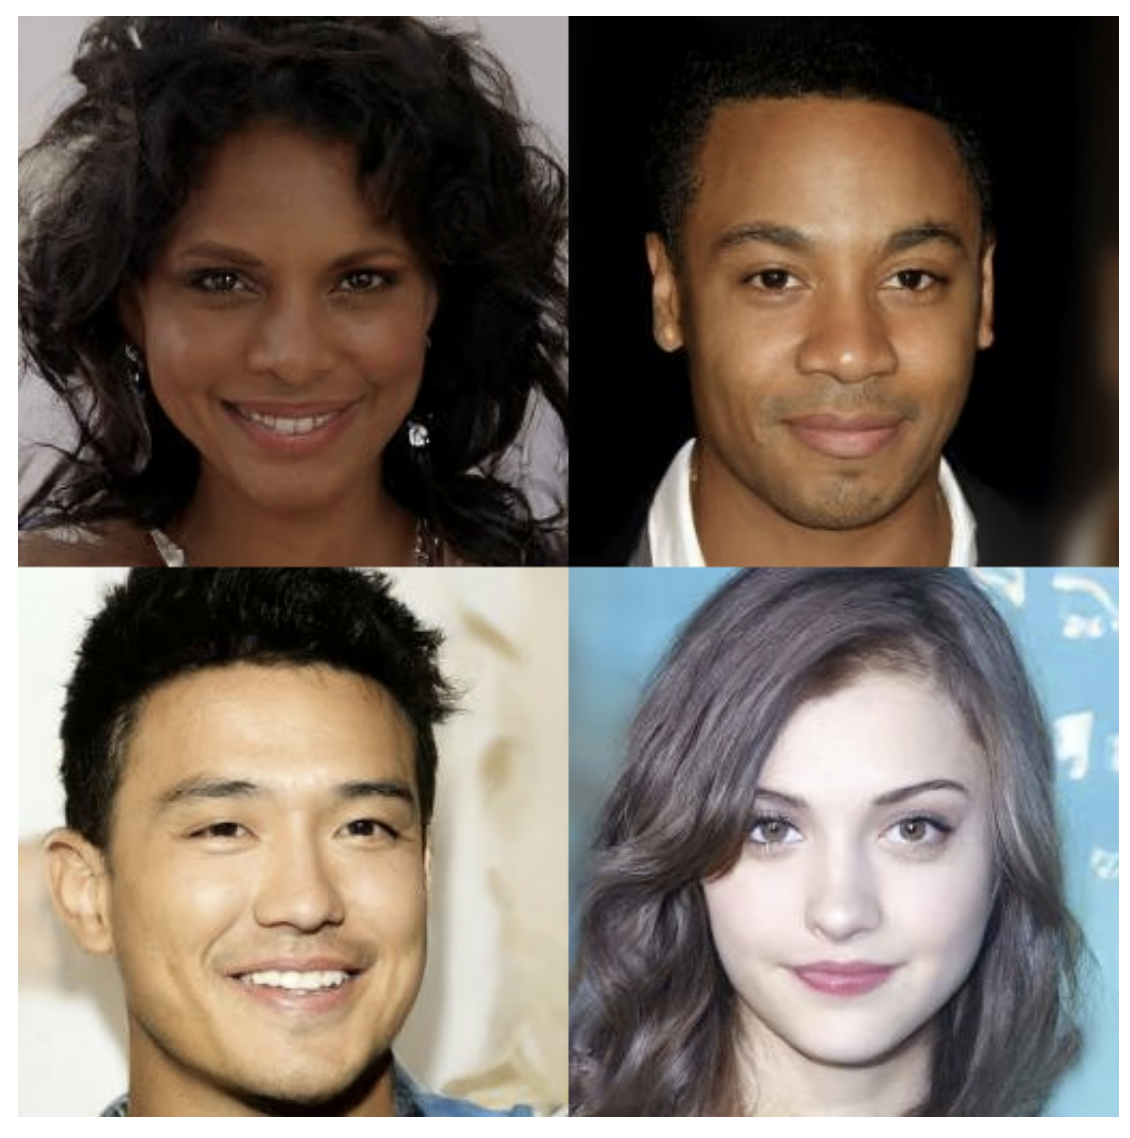
\includegraphics[width = 4in]{\images/DiffCeleb}}

\slide{Progressive VAEs}

Diffusion models are a special case of progressive VAEs.

\vfill
A progressive VAE has layers of latent variables $z_1,\dots,z_{L}$.

\vfill
It is not clear whether the diffusion model is the best way to do this.

\vfill
It could be that the important idea is simply having large $L$ with
$I(z_0,z_\ell)$ going from $H(z_0)$ to 0 as $\ell$ goes from $0$ to $L$.


\slide{Progressive VAEs}

A progressive VAE has layers of latent variables $z_1,\dots,z_{L}$.

\vfill
It seems more natural for image modeling to have spacial resolution decline with increasing $\ell$.

\vfill
This should eliminate the need for U-Nets and reduce computational cost.

\slide{END}
}
\end{document}
